\subsection{Цель работы}
Определить возможные структуры комплексов пропанола с молекулой воды и энергии образующейся при этом водородной связи.


\subsection{Постановка задач}
Предположить возможные комплексы молекул пропанола с водой, провести оптимизацию методом RHF/STO-3G и привести следующие результаты: 
\begin{itemize}
    \item число действительно различных комплексов с водородной связью;
    \item для каждого комплекса -- энергию водородной связи;
    \item наиболее энергетически выгодный комплекс и соответствующее значение водородной связи.
\end{itemize}

\begin{figure}[H]
\centering
\captionsetup{justification=centering}
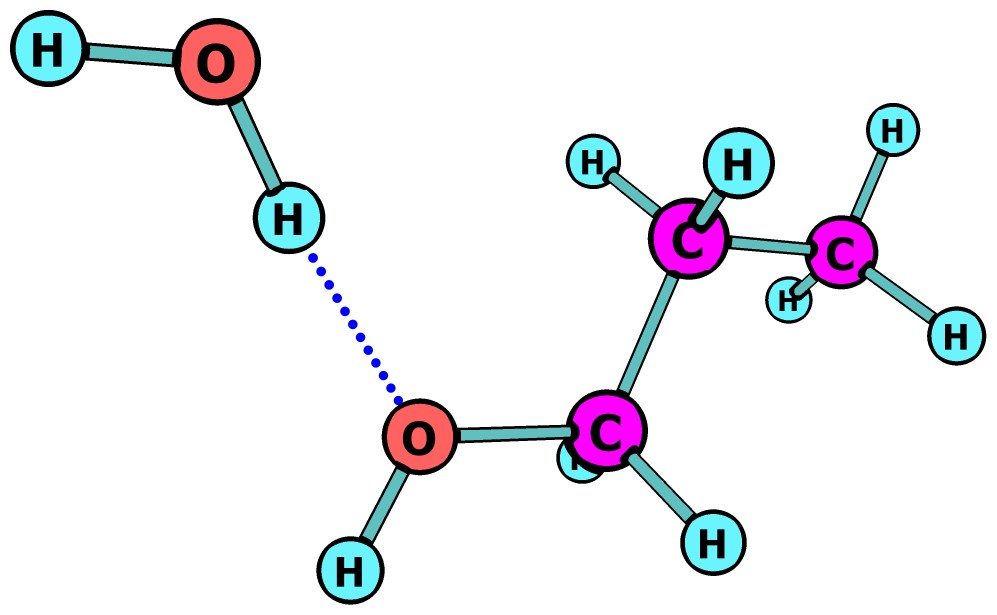
\includegraphics[scale=0.4]{fig/0.jpg}
\caption{Один из предложенных комплексов пропанола с молекулой воды.}
\end{figure}


\subsection{Теоретическая информация}
\subsubsection{Водородная связь}
Водородная связь — форма ассоциации между электроотрицательным атомом и атомом водорода H, связанным ковалентно с другим электроотрицательным атомом. В качестве электроотрицательных атомов могут выступать N, O или F. Энергия водородной связи, как правило, по абсолютной величине находится в пределах (0.003 - 0.022) Хартри.

\begin{figure}[H]
\centering
\captionsetup{justification=centering}
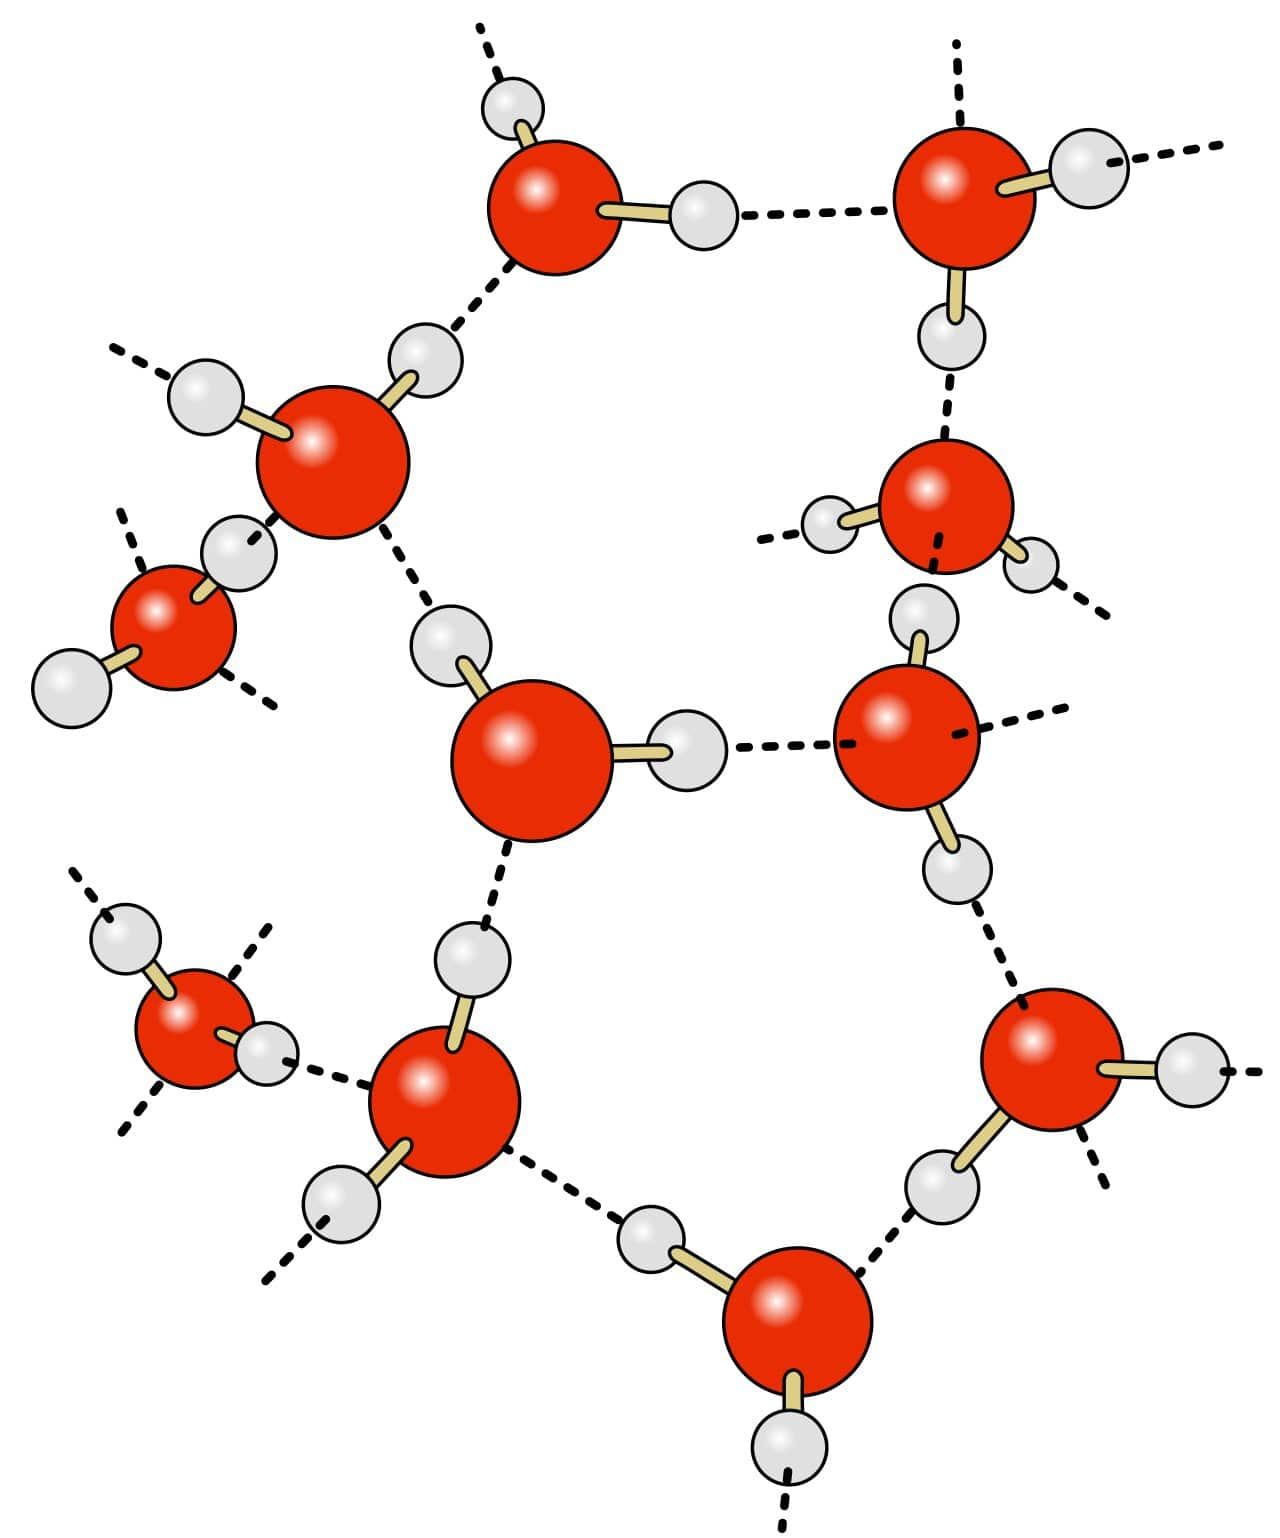
\includegraphics[scale=0.2]{fig/1.jpg}
\caption{Водородная связь между молекулами воды (чёрные пунктирные линии).}
\end{figure}


\subsection{Результаты}
Было предложено 5 различных комплексов. После проведения оптимизации были получены два стабильных различных комплекса. Информация о данных комплексах приведена в таблице ниже: 

\begin{table}[H]
\caption{Составляющие энергии комплексов} \label{tab:my-table}
\begin{center}
\resizebox{\textwidth}{!}{%
\begin{tabular}{|c|c|c|c|c|}
\hline
№ комплекса & Описание комплекса & \begin{tabular}[c]{@{}c@{}}Полная энергия\\ комплекса, Хартии\end{tabular} & \begin{tabular}[c]{@{}c@{}}Полная энергия \\ невзаимодействующего\\ комплекса, Хартри\end{tabular} & \begin{tabular}[c]{@{}c@{}}Энергия водородной\\ связи, Хартии\end{tabular} \\ \hline
1 & \begin{tabular}[c]{@{}c@{}}Водородная связь между\\ O2 и H1\end{tabular} & -265.688 & -265.678 & 0.01 \\ \hline
2 & \begin{tabular}[c]{@{}c@{}}Водородная связь между\\ O1 и H3\end{tabular} & -265.687 & -265.678 & 0.009 \\ \hline
\end{tabular}%
}
\end{center}
\end{table}

Более стабильным оказался первый комплекс.

\begin{figure}[H]
\centering
\captionsetup{justification=centering}
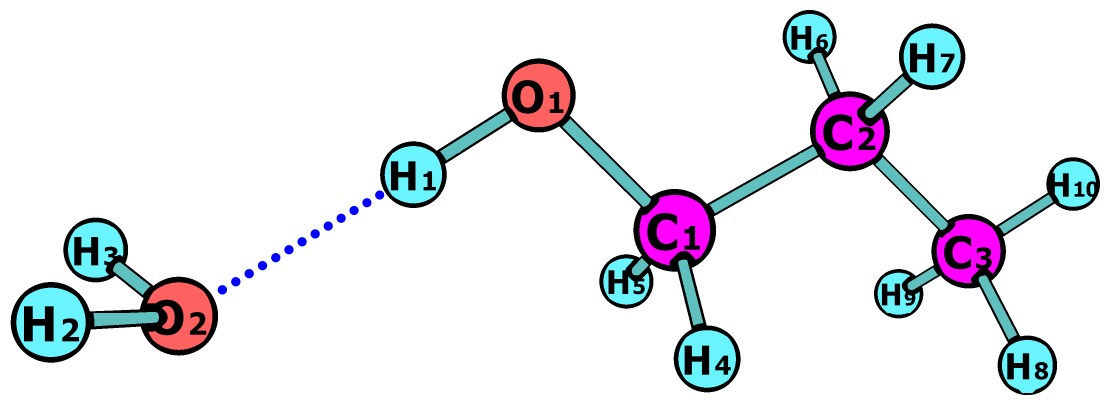
\includegraphics[scale=0.3]{fig/2.jpg}
\caption{Комплекс №1.}
\end{figure}

\begin{figure}[H]
\centering
\captionsetup{justification=centering}
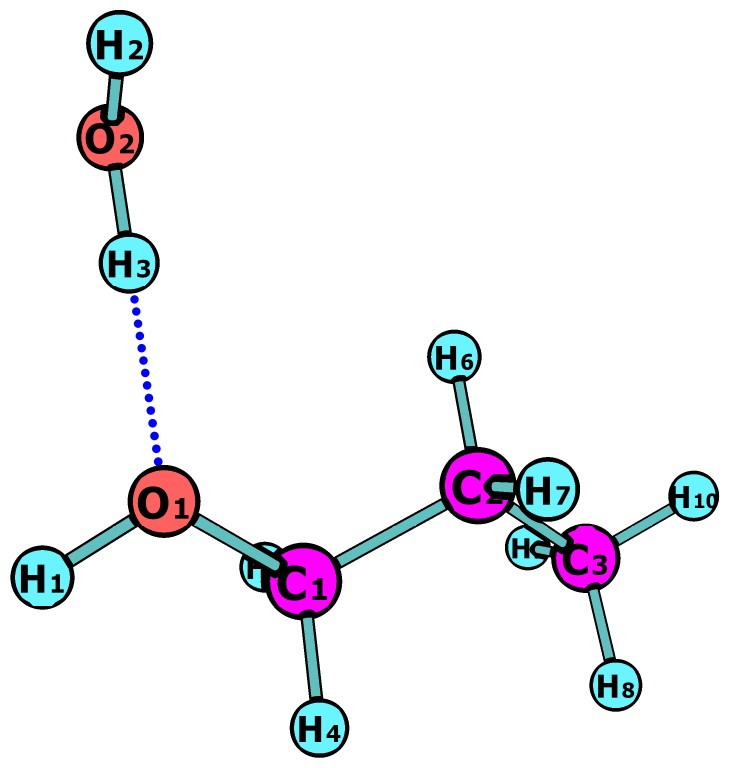
\includegraphics[scale=0.3]{fig/3.jpg}
\caption{Комплекс №2.}
\end{figure}


\subsection{Выводы}
Полученное значение энергии водородной связи для двух соединений находится в допустимом пределе: (0.003 - 0.022) Хартри. Оба комплекса являются стабильными и в растворе могут быть присутствовать оба комплекса.


\subsection{Контроль результатов}

\begin{itemize}
    \item у каждого рассматриваемого комплекса в выходном файле содержится “EQUILIBRIUM GEOMETRY LOCATED”;
    \item из пяти предложенных конформеров были обнаружены тождественные: энергия совпадает до 4 знака после запятой, геометрии тождественны; 
    \item значения энергий водородной связи находятся в допустимых пределах.
\end{itemize}{}


\subsection{Приложенные файлы}
\begin{itemize}
    \item complex\_origin.xyz – исходная структура невзаимодействующего комплекса;
    \item файлы в папке input – файлы на вход GAMESS;
    \item файлы в папке output – выходные файлы GAMESS.
\end{itemize}{}